\subsection{\DSp}
\label{sec:Proto}

%---
\subsection{Prototype Overview and Status}
The objective of the \DSps\ experiment is the construction and operation of a prototype detector of intermediate size (\DSpApproximateMass), to fully validate the new \DSks\ technologies for their integrity in both the mechanical and functional aspects.  The prototype will be constructed using the materials planned before screening, in order to speed up the mechanical validation, and will therefore not necessarily be a physics-results oriented detector. This may evolve over time to include elements of the detectors as materials are screened and made available, and eventually all parts could be replaced with radio pure materials to form the basis of another experiment with high-sensitivity to low-mass \WIMPs.  Thus, \DSps\  is not intended to replace validation and tests made in laboratories, but rather complement them with the integration with the rest of the detector.  The prompt execution of \DSps\ is crucial to fulfill the overall schedule of \DSks.  \DSps\ is on the critical path of the project.

The program for \DSps\ is expected to span over three different phases:
\begin{compactenum}
\item Design, construction and assembly at test site of the \LArTPC, with the size available for two motherboards integration;
\item Integration of \DSpZeroPdmsNumber\ preproduction \DSkPdms\ to the \LArTPC; assembly, commissioning, and operation of full read-out and DAQ for \DSpZeroPdmsNumber\ \DSkPdms; The $x y$ resolution and \STwo\ gas pocket optimization will be done during this phase.
\item Assembly and commissioning of full system, including \DSpPdmsNumber\ first production PDMs; full readout and DAQ operational; evolution towards final configuration. 
\end{compactenum}

The plan for \DSps\ was reviewed, approved, and funded by the CNS2 of INFN. Funding has already been secured from the NSF for the development and fabrication of multiple components for the \TPC, the cryogenics system and resources for kick-starting the \UAr\ extraction site preparations.  Requests for funding from other participating groups are being evaluated or will be submitted in the near future.

In August 2017 the collaboration and \LNGS\ reached and finalized an agreement \cite{Mapelli:2017vn} with the Accelerator \& Technology Sector of \CERN\ and its Technical Division to construct and commission the \DSks\ cryogenics at \CERN, with support from the Cryogenics Group and the Vacuum, Surfaces and Coatings Group (both groups are part of CERN's Technical Division). The extension of this program to carry out the first surface operation of \DSps\ at \CERN\ before moving the detector to \LNGS\ was agreed by the \CERN\ Accelerator \& Technology Sector via an Addendum to the above agreement. The necessary space and facilities are the same as for the test on the \DSk\ cryogenics and are already allocated.

A cryostat for \DSps\ has been built by Tecno Alarm, s.r.l., Roma, and delivered to \CERN\ in August 2018 (see Figure~\ref{fig:proto-cern}).  The \DSlCryostatUCont\ U/Th AISI 304 L Stainless Steel was procured from NIRONIT Edelstahlhandel GmbH \& Co and it is good enough to be used for a possible physics run in \LNGS.

\begin{figure}[!t]
\centering
\includegraphics[width=\columnwidth]{./Figures/CERN-ProtoLab.JPG}
\caption[The \DSps\ cryostat and components delivered at CERN]{The \DSps\ cryostat and components delivered at CERN.}
\label{fig:proto-cern}
\end{figure}

Assembly and test of the \DSks\ cryogenics will take place at \CERN, during the summer and last quarter of 2019. Construction of \DSps\ is expected at the end of 2019 or early 2020. The first test operation with a reduced number of photosensors is expected by summer 2019, followed by a second operation with a full complement of \DSkPdms\ by early 2020. Full characterization of the prototype performance and physics runs will be performed after installation at LNGS. The detailed program of the activities to be carried out underground is under study.

We anticipate that, since the \DSps\ will be a stand alone system, sharing the \DSks\ cryogenics system at \LNGS\ will not be possible. However over the past few years of R\&D for the \DSks\ cryogenics, we have realized and tested several key components which will be more than capable of handling the prototype system. These parts can be used for \DSps\ with minor system integration together with most of the \DSfs\ and existing R\&D devices.

\subsubsection{The \DSps\ \TPC}

The \DSps\ \TPC\ mechanics, including the structural elements, the field cage, the reflector cage, the transparent cathode, the transparent anode (also serving as a diving bell for the containment of the gaseous phase), the \SiPM\ \DSkPdm\ assemblies, the high-voltage feed through system, will all be built utilizing, on a scaled down overall dimension, the same design and construction techniques foreseen for the baseline of \DSks\ (see Figure~\ref{fig:proto_1ton}). 

\begin{figure}[!t]
\centering
%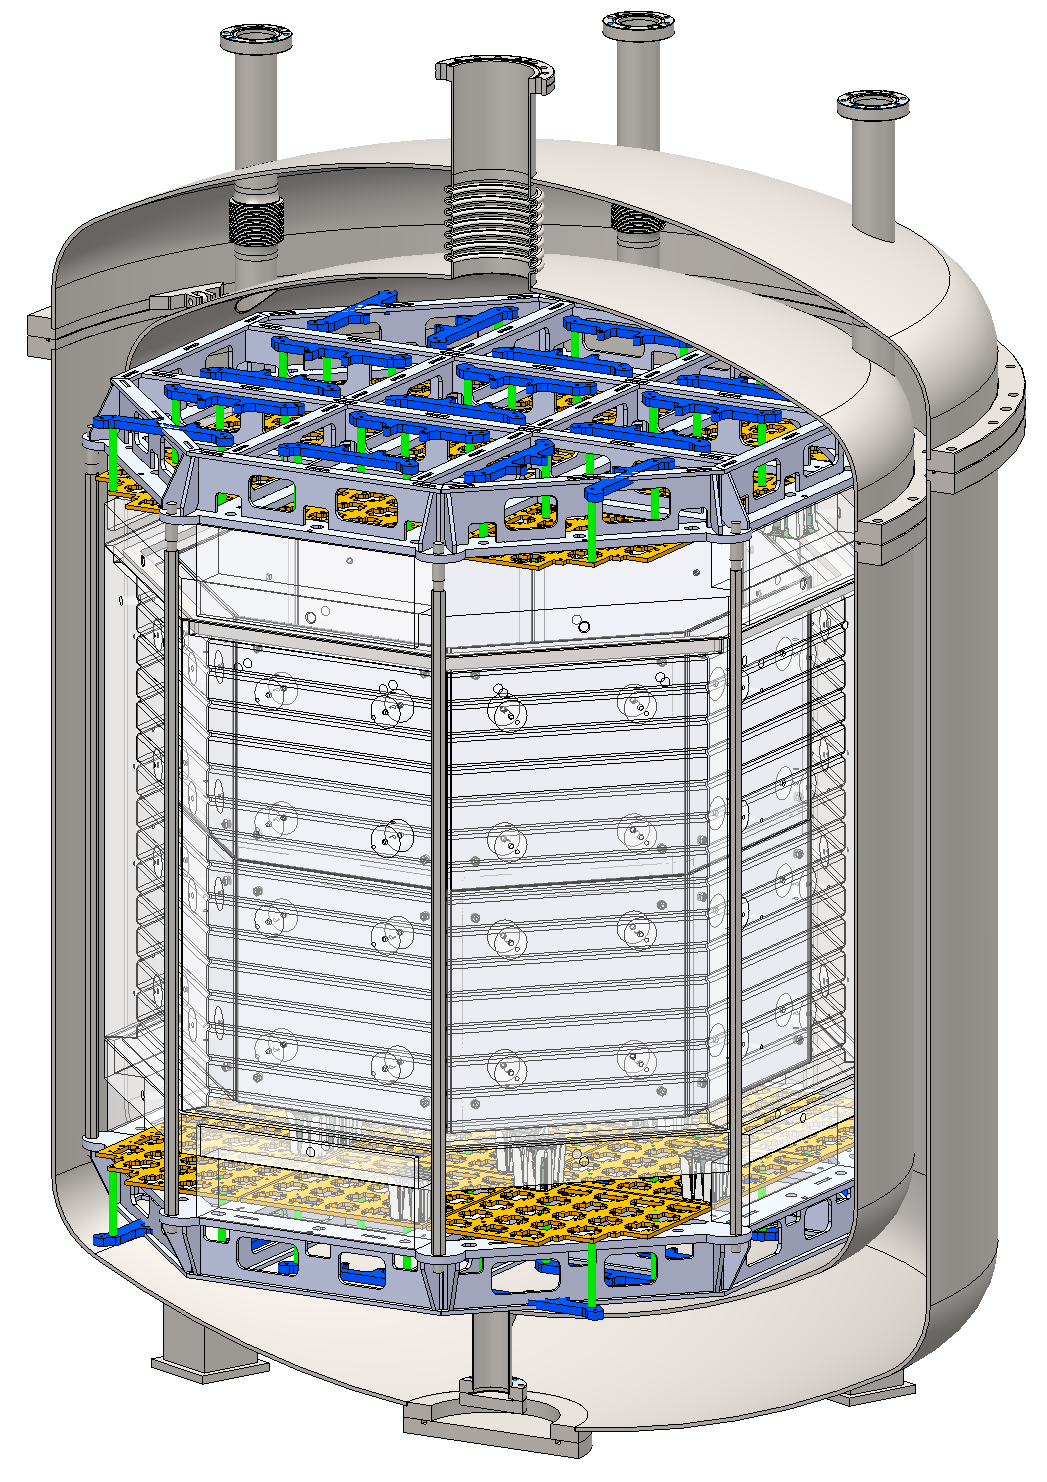
\includegraphics[height=0.95\textheight]{./Figures/proto_1ton.png}
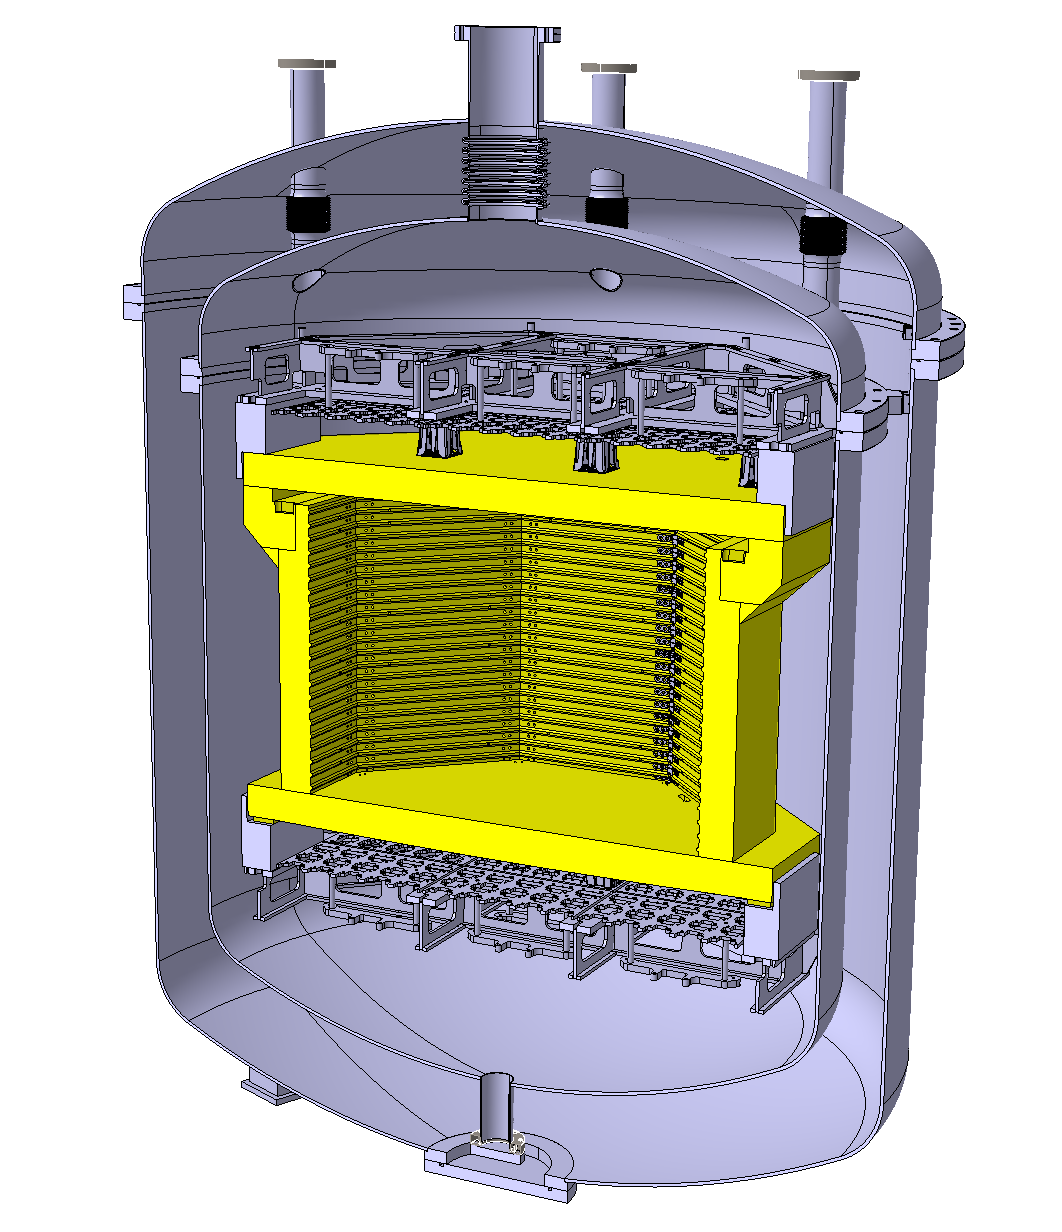
\includegraphics[width=0.98\textwidth]{./Figures/proto_1ton_newdesign_crop.png}
\caption[Conceptual design of the \DSps\ detector]{Conceptual Design of the \DSps\ detector.  The cryostat has already been built and delivered at \CERN, see \reffig{proto-cern}.}
\label{fig:proto_1ton}
\end{figure}

The photodetector modules will be arranged to cover the top and bottom of the \TPC. Both top and bottom planes consist of \DSpPdmsHalfNumber\ photodetector modules assembled into \DSpSQBsNumber\ \SQBs\ and \DSpTRBsNumber\ \TRBs. As described in section~\ref{sec:DAQ}, the readout chain will employ commercial components used during the first phase, allowing for full digitization of the signals.  The final electronics components that will be used in \DSks\ will be used as they become available at each stage of the development. It is also foreseen that the optical signal transmission will be tested on a significant number of channels with this detector.

The \DSps\ photosensors are contained in \DSpMBNumber\ Motherboards made of one set of \DSpSQBsNumber\  (\SQB) and \DSpTRBsNumber\  (\TRB) \DSkPdms\ on top, and another identical set on bottom.  With both planes, the \DSps\ \TPC\ requires \DSpPdmsNumber\ \DSkPdm\ to be fully covered. Bonding \DSpSipmsNumber\ \SiPMs\ in a few months is one of the most critical tasks of this detector, to maintain the overall project schedule. %The NOA facility will not be operative before summer 2019, while the schedule foresees a delivery of the \DSpMBNumber\ Motherboards by the end of 2019.
%The production of the \SiPMs\ by the LFoundry company requires a technological transfer from the FBK company. The time schedule agreed between the two companies foresees the delivery of the first \SiPMs\ by the end of February 2019.
%The time window available to bond the \DSpPdmsNumber\ tiles stays therefore between the devil and the deep blue: on one side the \SiPMs\ will not be available before February 2019 while on the other side the NOA personnel have to start their equipment learning by fall 2019, that includes periods spent in the company headquarters.
The construction strategy relies on two bonding facilities, the first one located at Princeton University and the second one at LNGS. According to the experience gained in the past months, a bonding rate of \DSpSipmsBondingRate\ is feasible.  We therefore need \DSpSipmsBondingTime\ to bond the \DSpPdmsNumber\ tiles across the two facilities.

The man power at \LNGS\ can be provided by the NOA contracts, while finding man power at Princeton University is more challenging. Different options were evaluated, and others are under consideration. The University of Manchester (UK) has identified a candidate who will spend a significant amount of time in the course of the next year to be trained, and then do the work.  A tight connection between the two production sites has to be provided, to include the harmonization of the procedures and quality assurance test. A person to provide this interface is being identified.  \LNGS\ requires a significant increase of man power since after the bonding the tiles will be equipped with a Front End Board (\FEB), and then mounted and tested at \LNGS. After the assembly, the tiles and the \FEB\ will be tested in \LIN.  The first Motherboard, made of \DSkSQBPdmsNumber\ \DSkPdms, was just assembled.  The Motherboard will be shipped to Napoli, where a comprehensive test at cryogenic temperature is scheduled.

A powerful test facility has to be prepared at Napoli, requiring extra man power. The procedures and the tools to ship the Motherboard from Pisa to Napoli and from Napoli to \CERN\ have to be carefully planned and made available. 


%---
\subsubsection{Materials for DarkSide-Proto}

Since \DSps\ is a test bench of \DSks, it won't be used to demonstrate the material radio-purity requirements of \DSks, however, it will be built with the goal of achieving the best radio-purity conceivable at the time of the construction, based on the current results of materials assay campaign. Additionally, \DSps\ can be used to assess the possible contamination related to the detector construction procedures (\TPC\ and PE), evidencing material cleaning/handling issues.

The assessment of the \DSps\ radioactive budget will be obtained through the material assay campaign and the Monte Carlo simulation. The validation of the predictions concerning the neutron/gamma originated by the material contamination will be only possible through data taken underground with the \DSps\ deployed in a properly shielded environment. A physics run, focused on the low-mass WIMP search, will be eventually possible with the \STwo-only analysis in the keV region. In this context, the minimization of the low-energy gamma background of the prototype will be extremely important to employ as early as possible.


%---
\subsubsection{Validation tests and operation}

Upon successful completion of the test phase of the different parts, we plan to measure the overall performance of the \DSps\ through some key parameters, such as the \SOne\ light yield, the electron drift time, electro-luminescence field and gas pocket thickness uniformity for high resolution of \STwo\ signals and the $x y$ position reconstruction. For the purpose of optimizing the \STwo\ signals, the first two Motherboards will be assembled into a small \TPC\ with reduced size drift length (\DSpZeroDriftLength) to avoid pile-up (see Figure~\ref{fig:mini-proto}). Full test of the \SOne\ response and therefore of the \SiPM\ readout chain can be obtained at the surface by switching off the electroluminescence field. The configuration of the gas pocket (geometry and field) can be varied by changing the distance between the anode and the wire grid, the width of the gas pocket, as well as the electro-luminescence field. The \STwo\ pulse shape can be precisely studied along with different gas pocket configurations, aiming to provide us the best solution for the future \LArTPC\ design.  This set-up will also allow for early studies of the \STwo\ formation and readout, to be carried out while the pre-production of the remaining Motherboards of the prototype is ongoing. The final set-up is shown in Fig.~\ref{fig:mini-proto}, equipped with two \DSkMBs. Currently a TPC equipped with only one mockup \DSkMB\ above the anode has been built and is undergoing test in \LAr. Upon completion of this first preliminary test a functioning \DSkMB\ equipped with pre-production \DSkPdms\ will be installed in the TPC and a first run will be performed to study specifically \STwo\ signal.

\begin{figure}[!t]
\centering
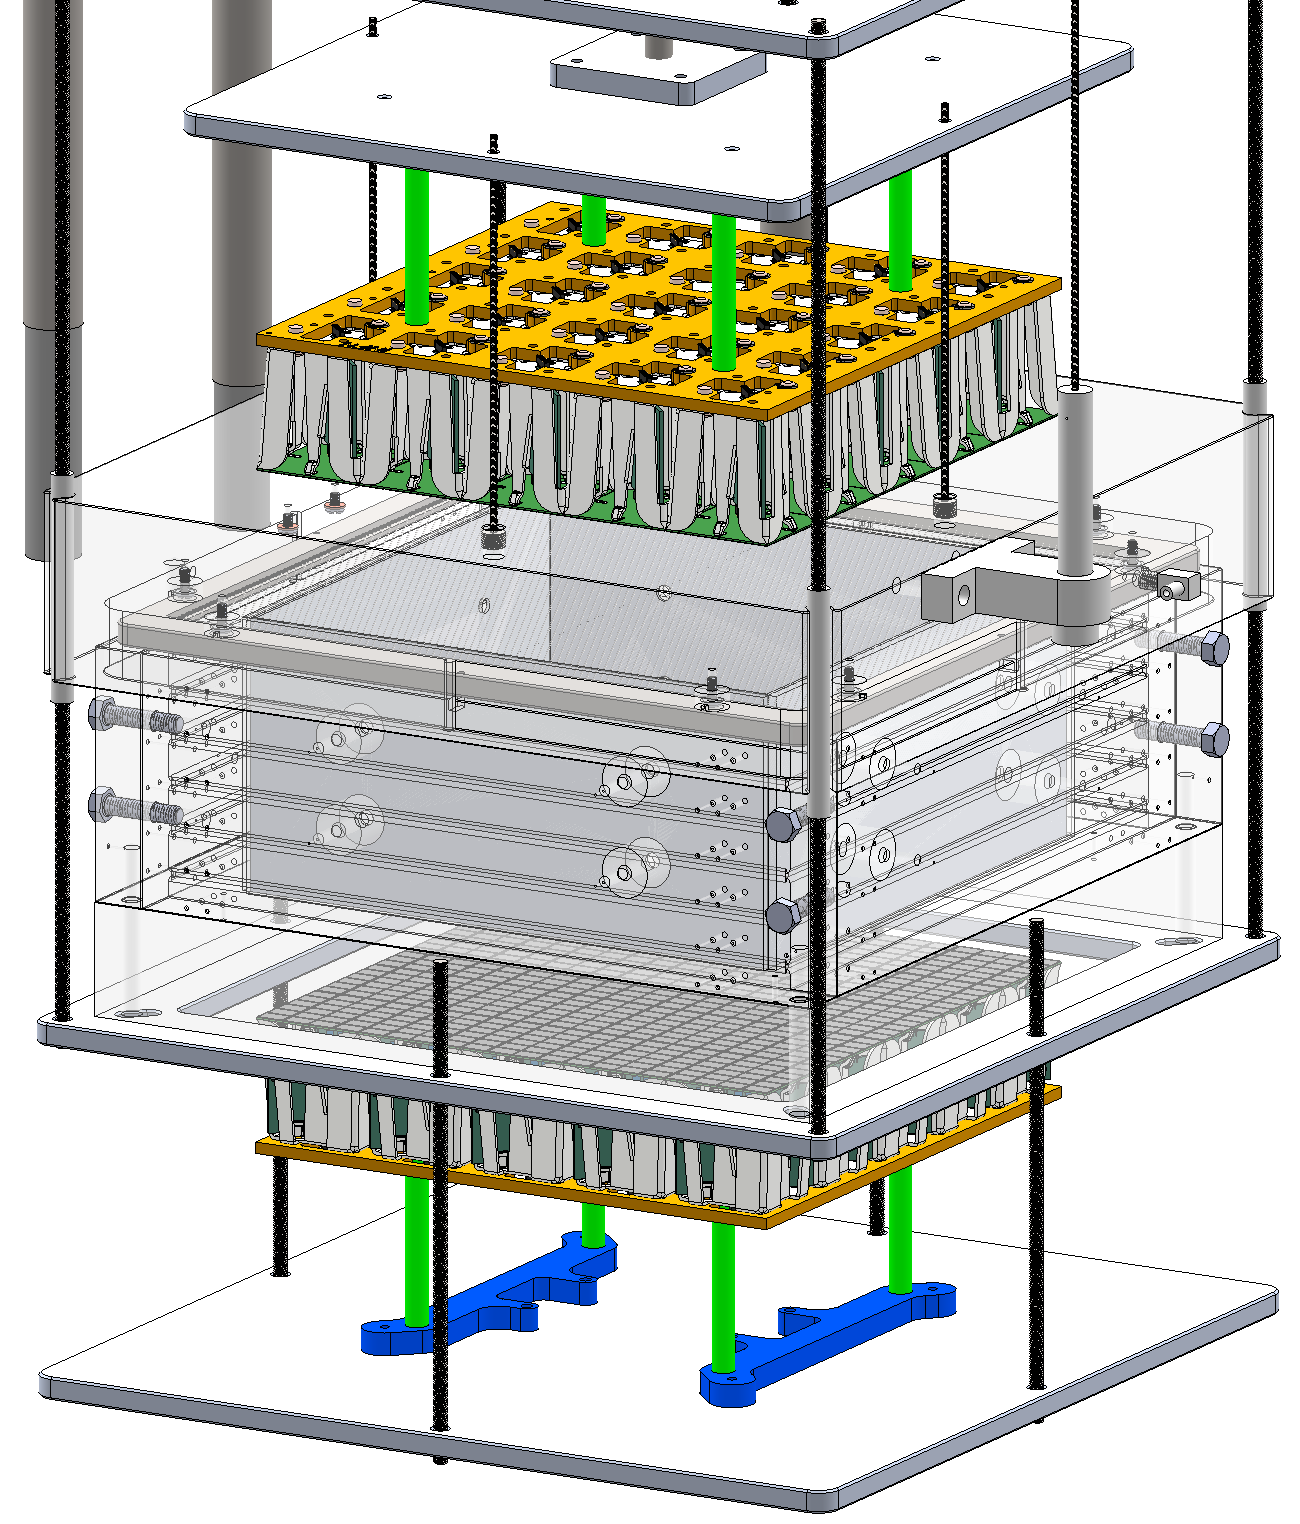
\includegraphics[height=0.8\textheight]{./Figures/mini-proto.png}
\caption[Schematics of the setup for the optimization of the \STwo\ signals]{Schematics of the setup for the optimization of the \STwo\ signals.}
\label{fig:mini-proto}
\end{figure}

\begin{figure}[!t]
\centering
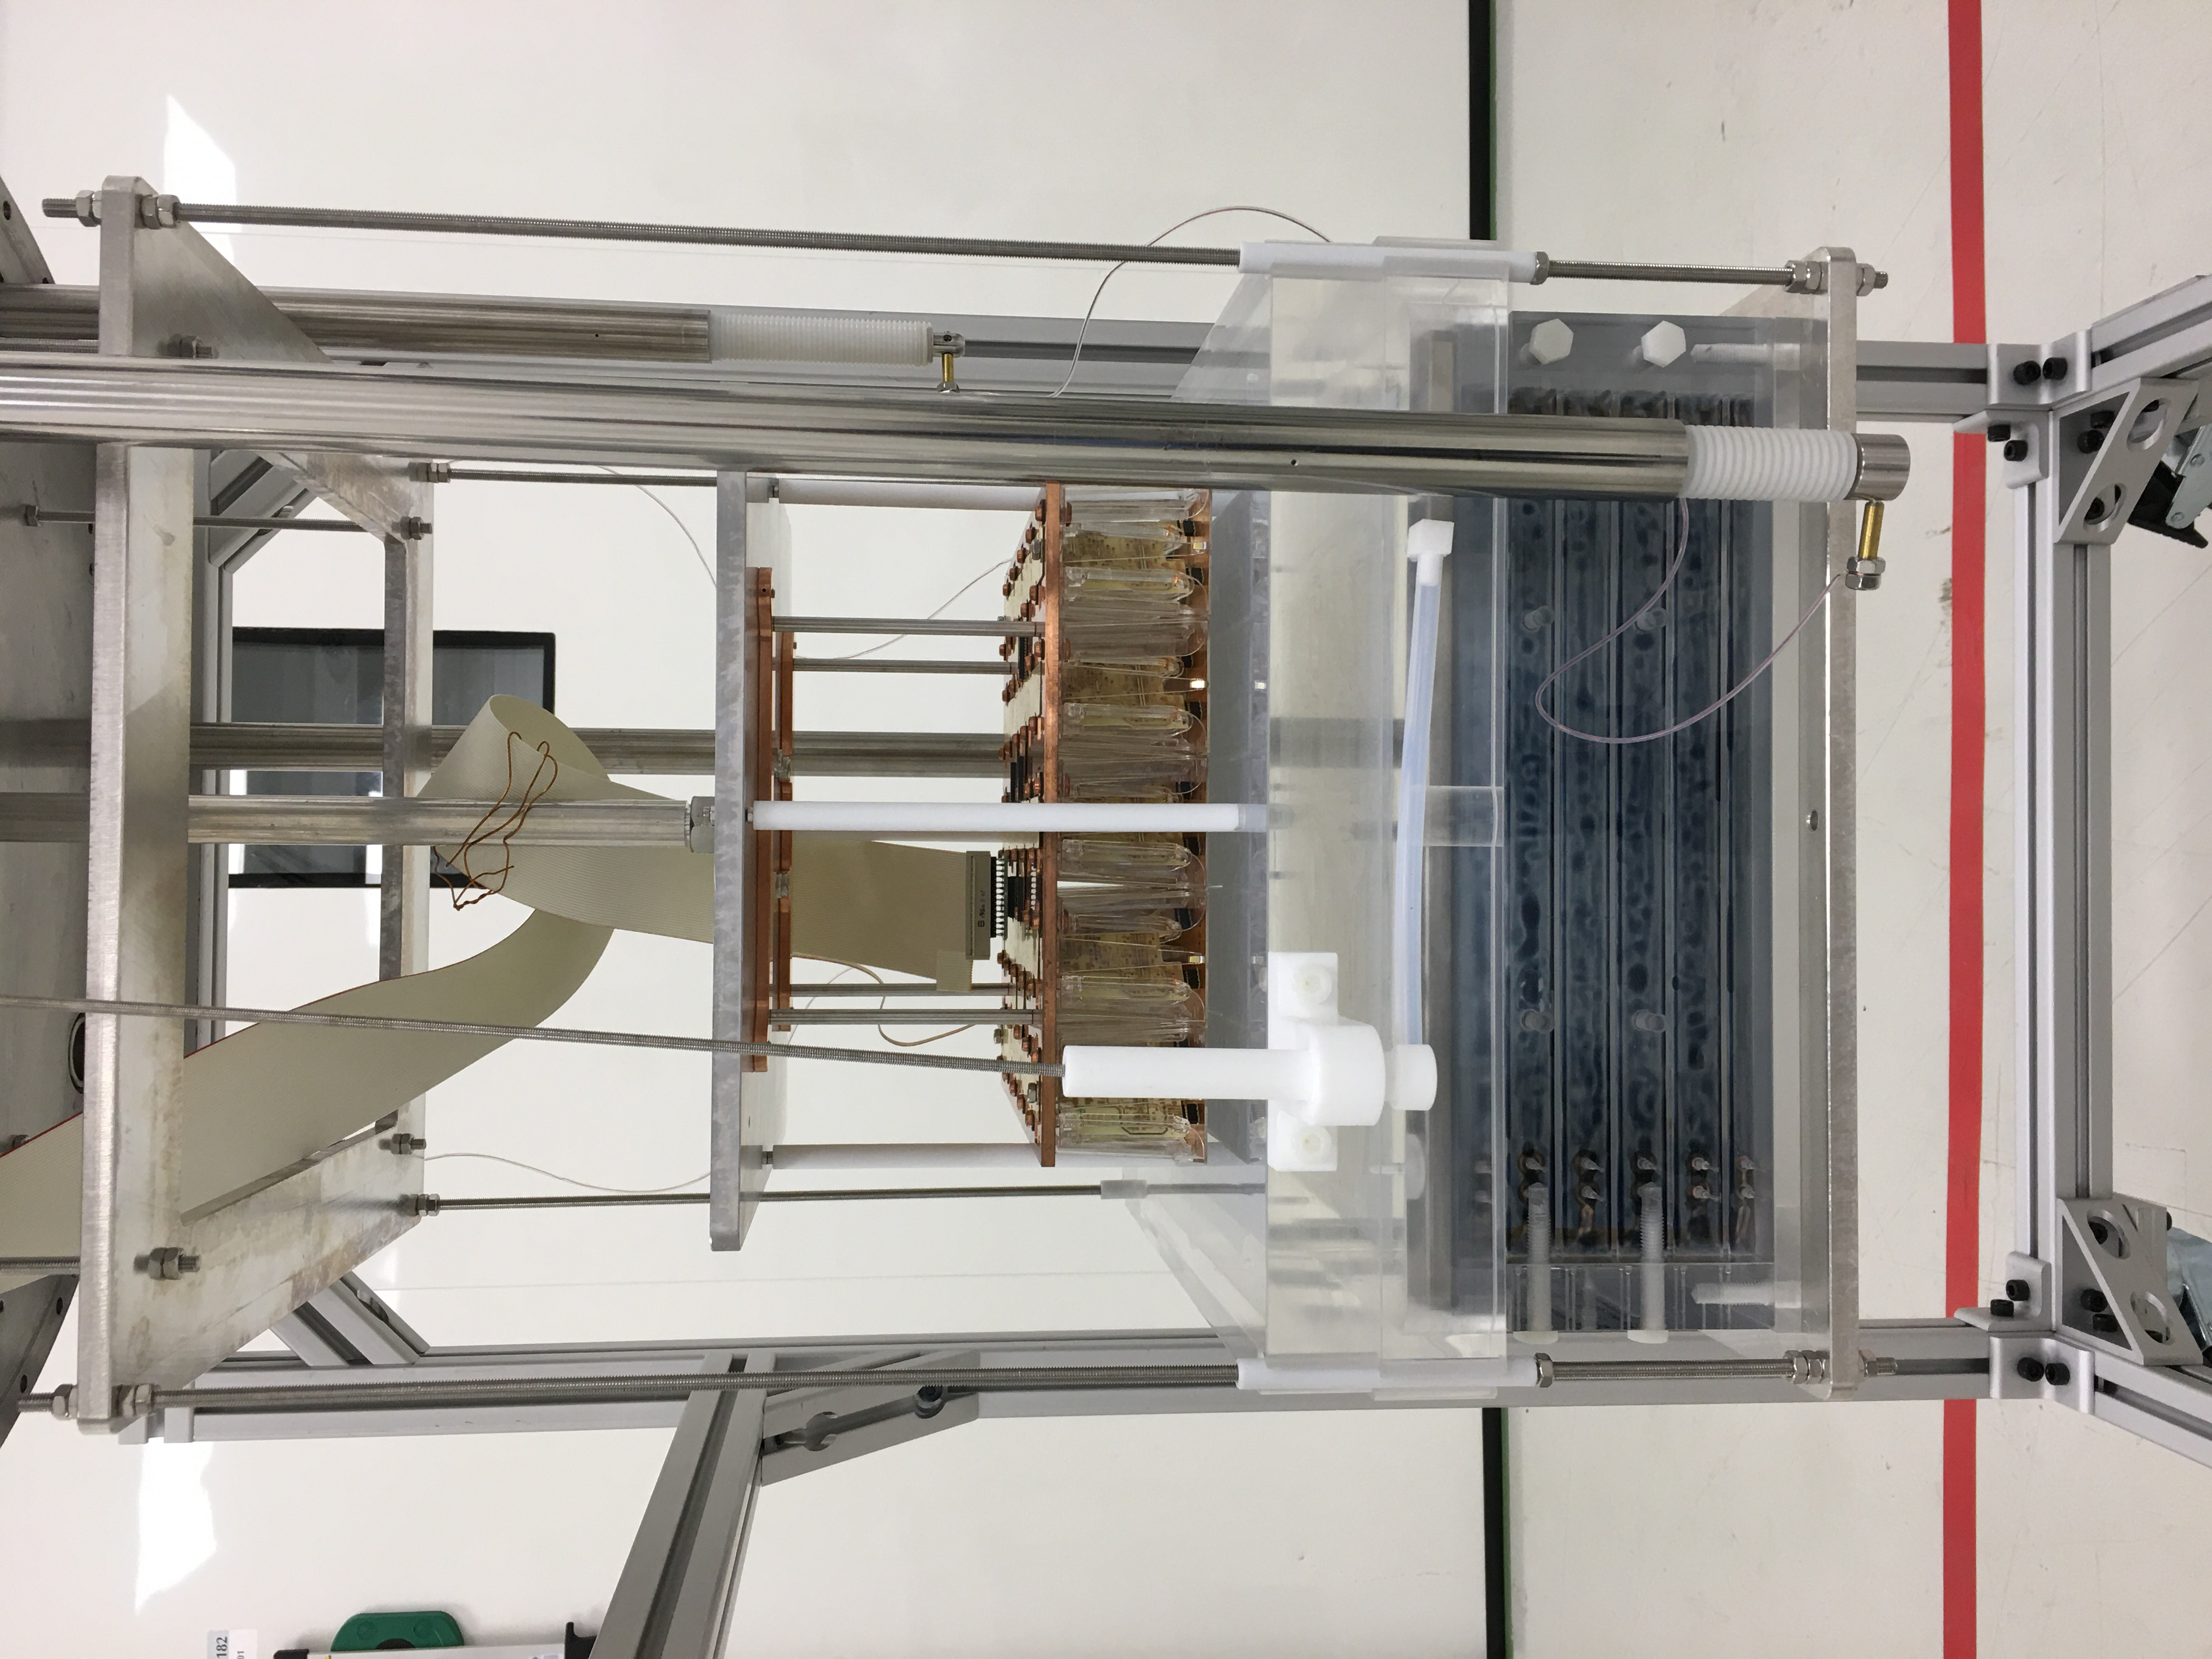
\includegraphics[angle=-90,width=0.8\textwidth]{./Figures/proto0_mockup.jpeg}
\caption[Picture of the mounted test TPC for the optimization of the \STwo\ signals.]{Picture of the mounted test TPC for the optimization of the \STwo\ signals.}
\label{fig:proto0_mockup}
\end{figure}